\documentclass{beamer}
\usepackage{algorithm}
\usepackage{algpseudocode}
\usepackage{graphicx}
\usepackage{amsmath}
\usepackage{hyperref}
\usepackage{float}
\usepackage{coffeestains}
\usepackage{authblk}
\usepackage{booktabs,siunitx}
\usetheme{Antibes}

\title{Risk aversion heterogeneity and contagion in
endogenous financial networks}
\bibliographystyle{apalike}
\author{Mateusz Dadej}
\institute{University of Brescia}
% write an affiliation

\date[VLC 2023] % (optional)
{Presentation of the research activity to the Scientific Board, 2023}

\begin{document}


\begin{frame}{Bank's balance sheet}

    \begin{itemize}
        \item The model build on works of Aldasoro et. al (2017) and Bluhm and Krahnen (2014). %\citet{bluhm} and \citet{aldasoro}
        \item It consists of $N$ banks, each with the balance sheet satisfying following identity:
        
        \[c_i + \underbrace{\sum_{j=1}^{N}l_{i,j}}_{l_i} + e_i = d_i + \underbrace{\sum_{j=1}^{N}b_{i,j}}_{b_i} + q_i\]

        \item Where asset side consists of cash $c$, external assets $e$ and interbank loans $l_{i,j}$. On the other side there are deposits $d$, interbank liabilities $l_{i,j}$ and equity $q_i$.
        
        % I guess we can set only $l_{i,j}$, and just reverse the indexation for the RHS
    \end{itemize}

\end{frame}

\begin{frame}{Financial network representation}

    \begin{itemize}
        \item The double indexation represents the interconectedness among banks. $l_{i,j}$ is the value of debt claim from bank $i$ to bank $j$.
        \item Therefore, $\sum_{j=1}^{N}l_{i,j}$ is a portfolio of claims of bank $i$
        \item These assets are not necessarily limited to interbank loans, but can also include other contracts that posses credit risk.
    \end{itemize}   

\end{frame}

\begin{frame}{Objective of banks}

    \begin{itemize}
        \item The profit function of banks depend on external and interbank assets and their return, respectively $r^e$ and $r^l$. As well as the cost of its funding, that depends on the default probability $\delta$ and loss given default $\zeta$.
        
        \[\pi_i = r_{i}^e e_i + r^l l_i - \left(\frac{1}{1 - \zeta \delta}\right) r^l b_i\]

        \item The utility function of a bank is a standard CRRA function
        
        \[U(\pi_i, \sigma_i) = \frac{\pi^{1-\sigma_i}}{1 - \sigma_i}\]


    \end{itemize}
    
\end{frame}

\begin{frame}{Objective of banks - expected utility}

    \[U(\pi_i) \approx U(E[\pi_i]) + U'((\pi_i - E[\pi_i])) + \frac{1}{2} U''((\pi_i - E[\pi_i])^2)\]

Taking the expected value of both sides:

\begin{equation}
  \begin{aligned}
    E[U(\pi_i)] &\approx E[U(E[\pi_i])] + U'(E[(\pi_i - E[\pi_i])]) + \frac{1}{2} U''(E[(\pi_i - E[\pi_i])^2]) \\
     &\approx U(E[\pi_i]) + \frac{1}{2} U''(\pi_i) \sigma^2_{\pi}
  \end{aligned}\nonumber
\end{equation}

The expected value of utility is following:

\[ E[U(\pi, \sigma_i, \sigma_\pi)] = \frac{\pi^{1-\sigma_i}}{1 - \sigma_i} - \frac{\sigma_i}{2} \pi^{-1-\sigma_i} \sigma_\pi\]

\end{frame}

\begin{frame}{Objective of banks - profit variance}
    Where $\sigma_i$ is the risk aversion of bank $i$ and $\sigma_\pi$ is the variance of the profit of bank $i$, given by:
        
    \begin{equation}
        \begin{aligned}
          \sigma^2_\pi &= V[r^e_i e_i + r^l l_i - \frac{1}{1 - \zeta \delta_i} r^l b_i] \\
          &= e_i^2 \sigma^2_{r^e_i} - (b_i r^l)^2 V[\frac{1}{1 - \zeta \delta_i}] + 2 e_i r^l \textbf{Cov}[r^e_i, \frac{1}{1 - \zeta \delta_i}]
        \end{aligned}\nonumber
      \end{equation}
      
      Taking the first order Taylor approximation around expected value of $\delta_i$:
      
      \[V[\frac{1}{1 - \zeta \delta_i}] = \zeta^2 (1 - \zeta E[\delta_i])^{-4} \sigma^2_{\delta_i}\]

      \[\sigma_\pi = e_i^2 \sigma_{r_i^e} - (b_i  r_l)^2  \zeta^2 (1 - \zeta \mathbf{E}[\delta])^{-4}  \sigma_\delta\]
      
\end{frame}

\begin{frame}{Regulatory requirements}

    \begin{itemize}
        \item Banks have to satisfy the following capital requirements:
        
        \[\frac{c_i + l_i + e_i - d_i - b_i}{\omega_e e_i + \omega_l l_i} \geq (\gamma + \tau)\]

        \item Where $\omega_e$ and $\omega_l$ are the weights of external and interbank assets, respectively. $\gamma$ is the minimum capital requirement and $\tau$ is the buffer.
        
        \item Additionally, banks are required to hold a minimum amount of liquid assets, relative to their deposits:
        
        \[c_i \geq \alpha \times d_i\]

    \end{itemize}

\end{frame}

\begin{frame}{Banks optimization problem}

    Each bank is deciding on the structure 

    \[\max_{c_i, e_i, l_i, b_i} \mathbf{E}[U(\pi_i, \sigma_i, \sigma_\pi)]\]

    S.t.:

    \[c_i + l_i + e_i = d_i + b_i + q_i\]

    \[\frac{c_i + e_i + l_i - d_i - b_i}{\omega_e e_i + \omega_l l_i} \geq (\gamma + \tau)\]
    
    \[c_i \geq \alpha \times d_i\]
        
\end{frame}

\begin{frame}{Interbank market}
    
    \begin{itemize}
        \item Both the interest at which the banks lend and borrow is in the equilibrium, that satisfy the condition:
        
        \[\sum_{i}^{N} l_i^* = \sum_{i}^{N} b_i^*\]
        
        \item Where $*$ are optimal amount of lending and borrowing for each bank.
        
        \item The interest satisfying the condition is obtained Iteratively, using the tâtonnement process (next slide). 
    \end{itemize}

\end{frame}

\begin{frame}{Tâtonnement process}
    
    \begin{algorithm}[H]
        \caption{tatonnement process}\label{alg:cap}
        \begin{algorithmic}
        \State $r^l \gets 0.05$
        \State $r^l_{max} \gets 0.1$
        \State $r^l_{min} \gets 0$
        \While{$|\Delta| < tol $}
        \State $\Delta \gets \sum_{i}^{N} l_i^* - \sum_{i}^{N} b_i^*$
        \If{$\Delta > 0$}
            \State $r^l_{max} \gets r^l$
            \State $r^l \gets \frac{r^l_{min} + r^l}{2}$
        \ElsIf{$\Delta < 0$}
            \State $r^l_{min} \gets r^l$
            \State $r^l \gets \frac{r^l_{max} + r^l}{2}$
        \EndIf
        \EndWhile
        \end{algorithmic}
    \end{algorithm}

\end{frame}

\begin{frame}{Matching funds}

Following linear program allows to match the funds among banks:

\begin{equation}
    \begin{aligned}
    \max_{A^{ib}_i} \quad & \sum_{i}^{N} \sigma_i (A^{ib}_i)^T k_i\\
    \textrm{s.t.} \quad & A^{ib}_{i,i} = 0 & \forall \; i \in N && \text{No self-lending}\\
      & A^{ib}_i \geq 0 & \forall \; i \in N && \text{No short-selling}\\
      & \sum_i^n A^{ib}_i = l_i & \forall \; i \in N && \text{Matching aggregated loans}\\
      & \sum_j^n A^{ib}_j = b_j & \forall \; j \in N && \text{Matching aggregated borrowing}\\ 
      & \frac{A^{ib}_i}{A^{\textbf{total}}_i} \leq \frac{1}{5} & \forall \; j \in N && \text{Maximum exposure limit}\\ 
    \end{aligned}
  \end{equation}
    
\end{frame}

\begin{frame}{Exogenous shock to the system}

    After setting the system in equilibrium, we introduce a shock in a form of a single random default. The process of defaulting is as follows:

    \begin{itemize}
        \item Defaulted bank repays the deposit with cash.
        \item If there are remaining deposits to be repaid, the bank is calling its interbank loans.
        \item Remainings from the called loans are distributed across interbank creditors.
        \item the rest of the debt is written down.
        \item Creditors with defaulted loans may have a negatie equity and are thus defaulting. 
    \end{itemize}
    
\end{frame}

\begin{frame}{Risk aversion heterogeneity}
    
    \begin{itemize}
        \item We want to inspect the effect of risk aversion heterogeneity on the contagion. 
        \item In other words, what is the effect on a system of a single bank with substantially different risk-apetite? 
        \item In order to do it, the following procedure is applied:
        
        \begin{equation}
            \begin{aligned}
              \sigma_{i \neq \textbf{ss}} = 2 + \frac{\Delta_{\textbf{ss}}}{N-1} \\ 
              \sigma_{\textbf{ss}} = 2 - \Delta_{\textbf{ss}}
            \end{aligned}\nonumber
        \end{equation}

    \end{itemize}

\end{frame}

\begin{frame}{Simulation parameters}

    \begin{table}
    \begin{center}
        \begin{tabular}{|c c|} 
         \hline
         Parameter & Value\\ [0.3ex] 
         \hline\hline
         $N$ & 20 \\ 
         \hline
         $\alpha$ & 0.01 \\
         \hline
         $\omega_e$ & 1 \\
         \hline
         $\omega_l$ & 0.2\\
         \hline
         $\tau$ & 0.01 \\ 
         \hline
         $\zeta$ & 0.6 \\ 
         \hline
         $E[\delta]$ & 0.005 \\
         \hline
         $\sigma_\delta$ & 0.003 \\ 
         \hline
         $r_e$ & $U(0, 0.15)$ \\ 
         \hline
         $V[r_e]$ & $\frac{1}{12}(\max(r^e) - \min(r^e))^2$ \\  [1ex] 
         \hline
        \end{tabular}
    \end{center}

    \

    Parameters were based on bank level balance sheet data (2019) from Orbis

\end{table}
    
    % \begin{itemize}
    %     \item The deposit and equity is taken from the balance sheet data of top 20 banks from the USA.
    % \end{itemize}

\end{frame}

\begin{frame}{Reproducing empirical data}

 
\begin{table}
    \begin{center}
        \begin{tabular}{|c | c | c|} 
         \hline
         Parameter & empirical value  & model value\\ [0.3ex] 
         \hline\hline
         $cash / deposits$ & $5.56\%$ &  $3.56\%$ \\ 
         \hline
         $\text{interbank lend.} / captial$ & $138.5\%$ &  $159.3\%$ \\
         \hline
         $\text{interbank lend.} / A$ & $15.29\%$ &  $22.17\%$ \\
         \hline
         $\text{capital} / A$ & $7.2\%$ &  $9.23\%$ \\
         \hline
         Average degree & NA & $2.8$ \\
         \hline
         $r^l$ & $-0.32\%$ & $2.24\%$ \\  [1ex] 
         \hline
        \end{tabular}
    \end{center}
\end{table}
    
\end{frame}

\begin{frame}{Simulation results I}
    
\begin{figure}[H]
    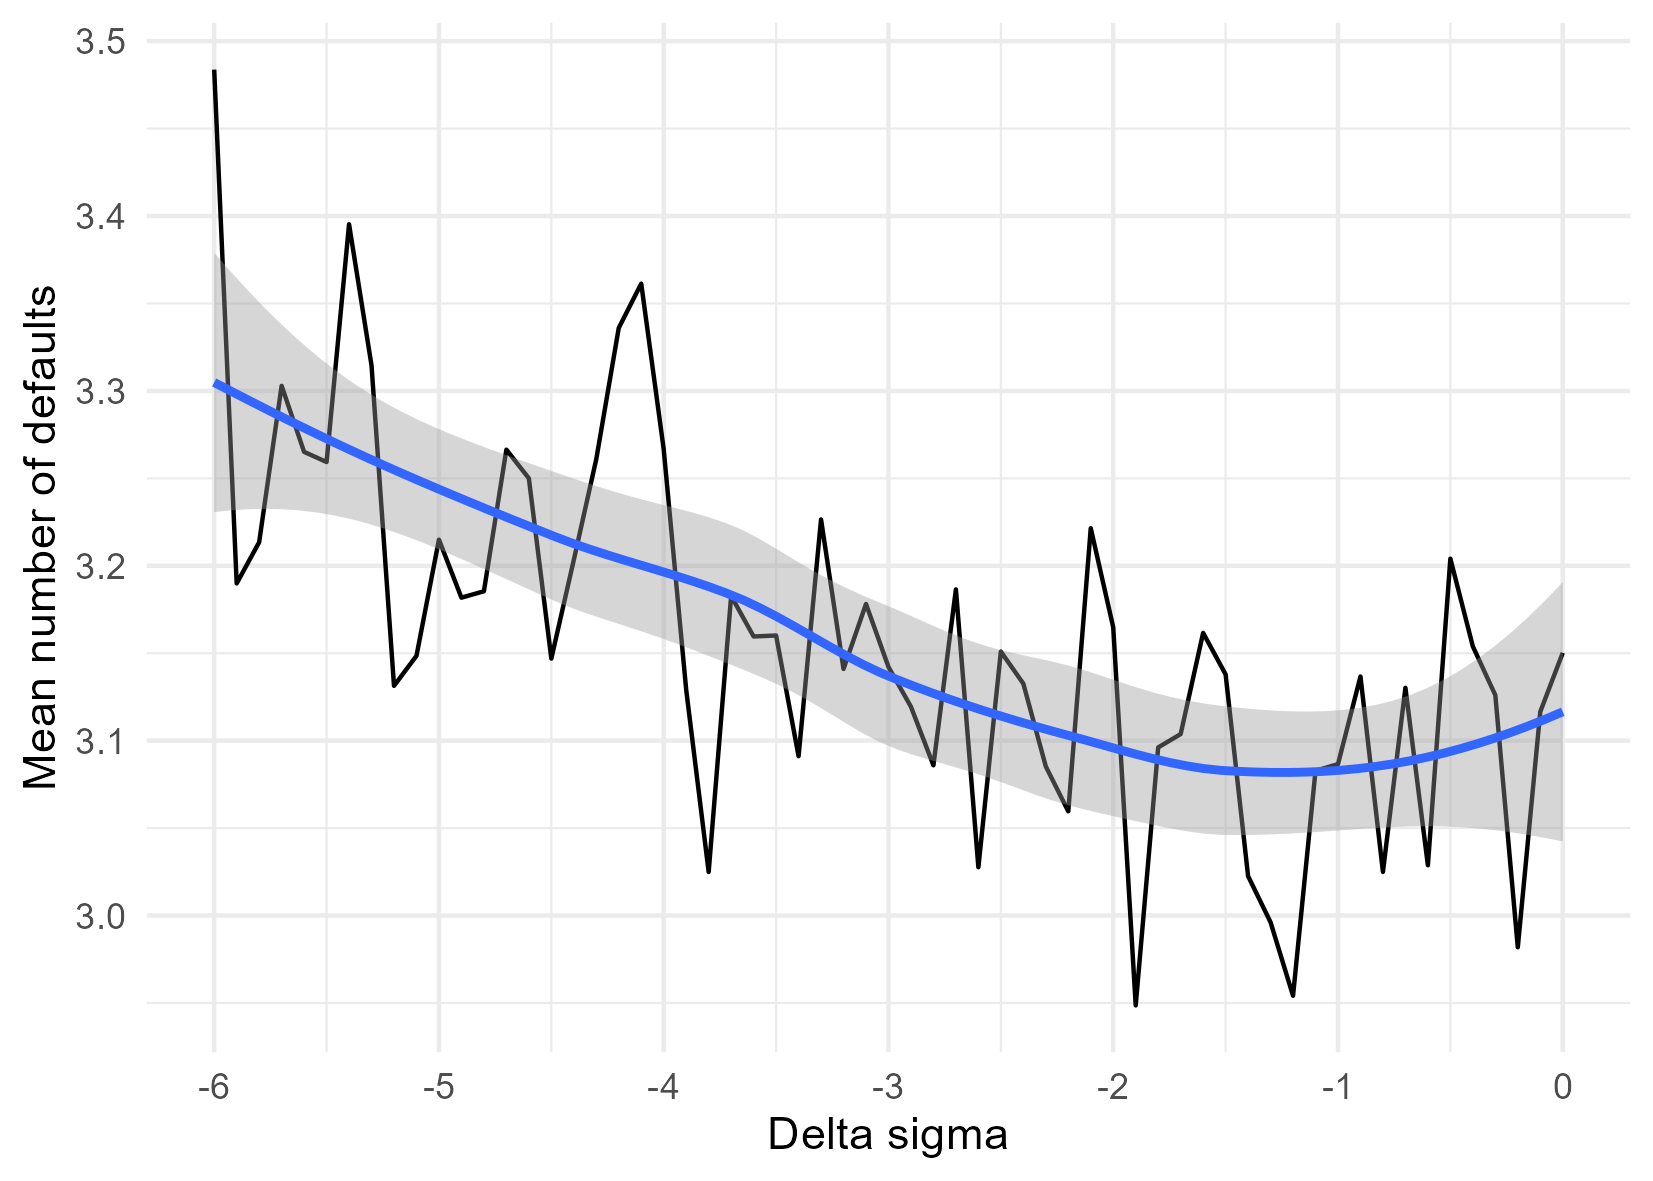
\includegraphics[scale=0.6]{delta_sigma.png}
    \centering
\end{figure}  
  
\end{frame}

\begin{frame}{Simulation results II}
    
    \begin{figure}[H]
        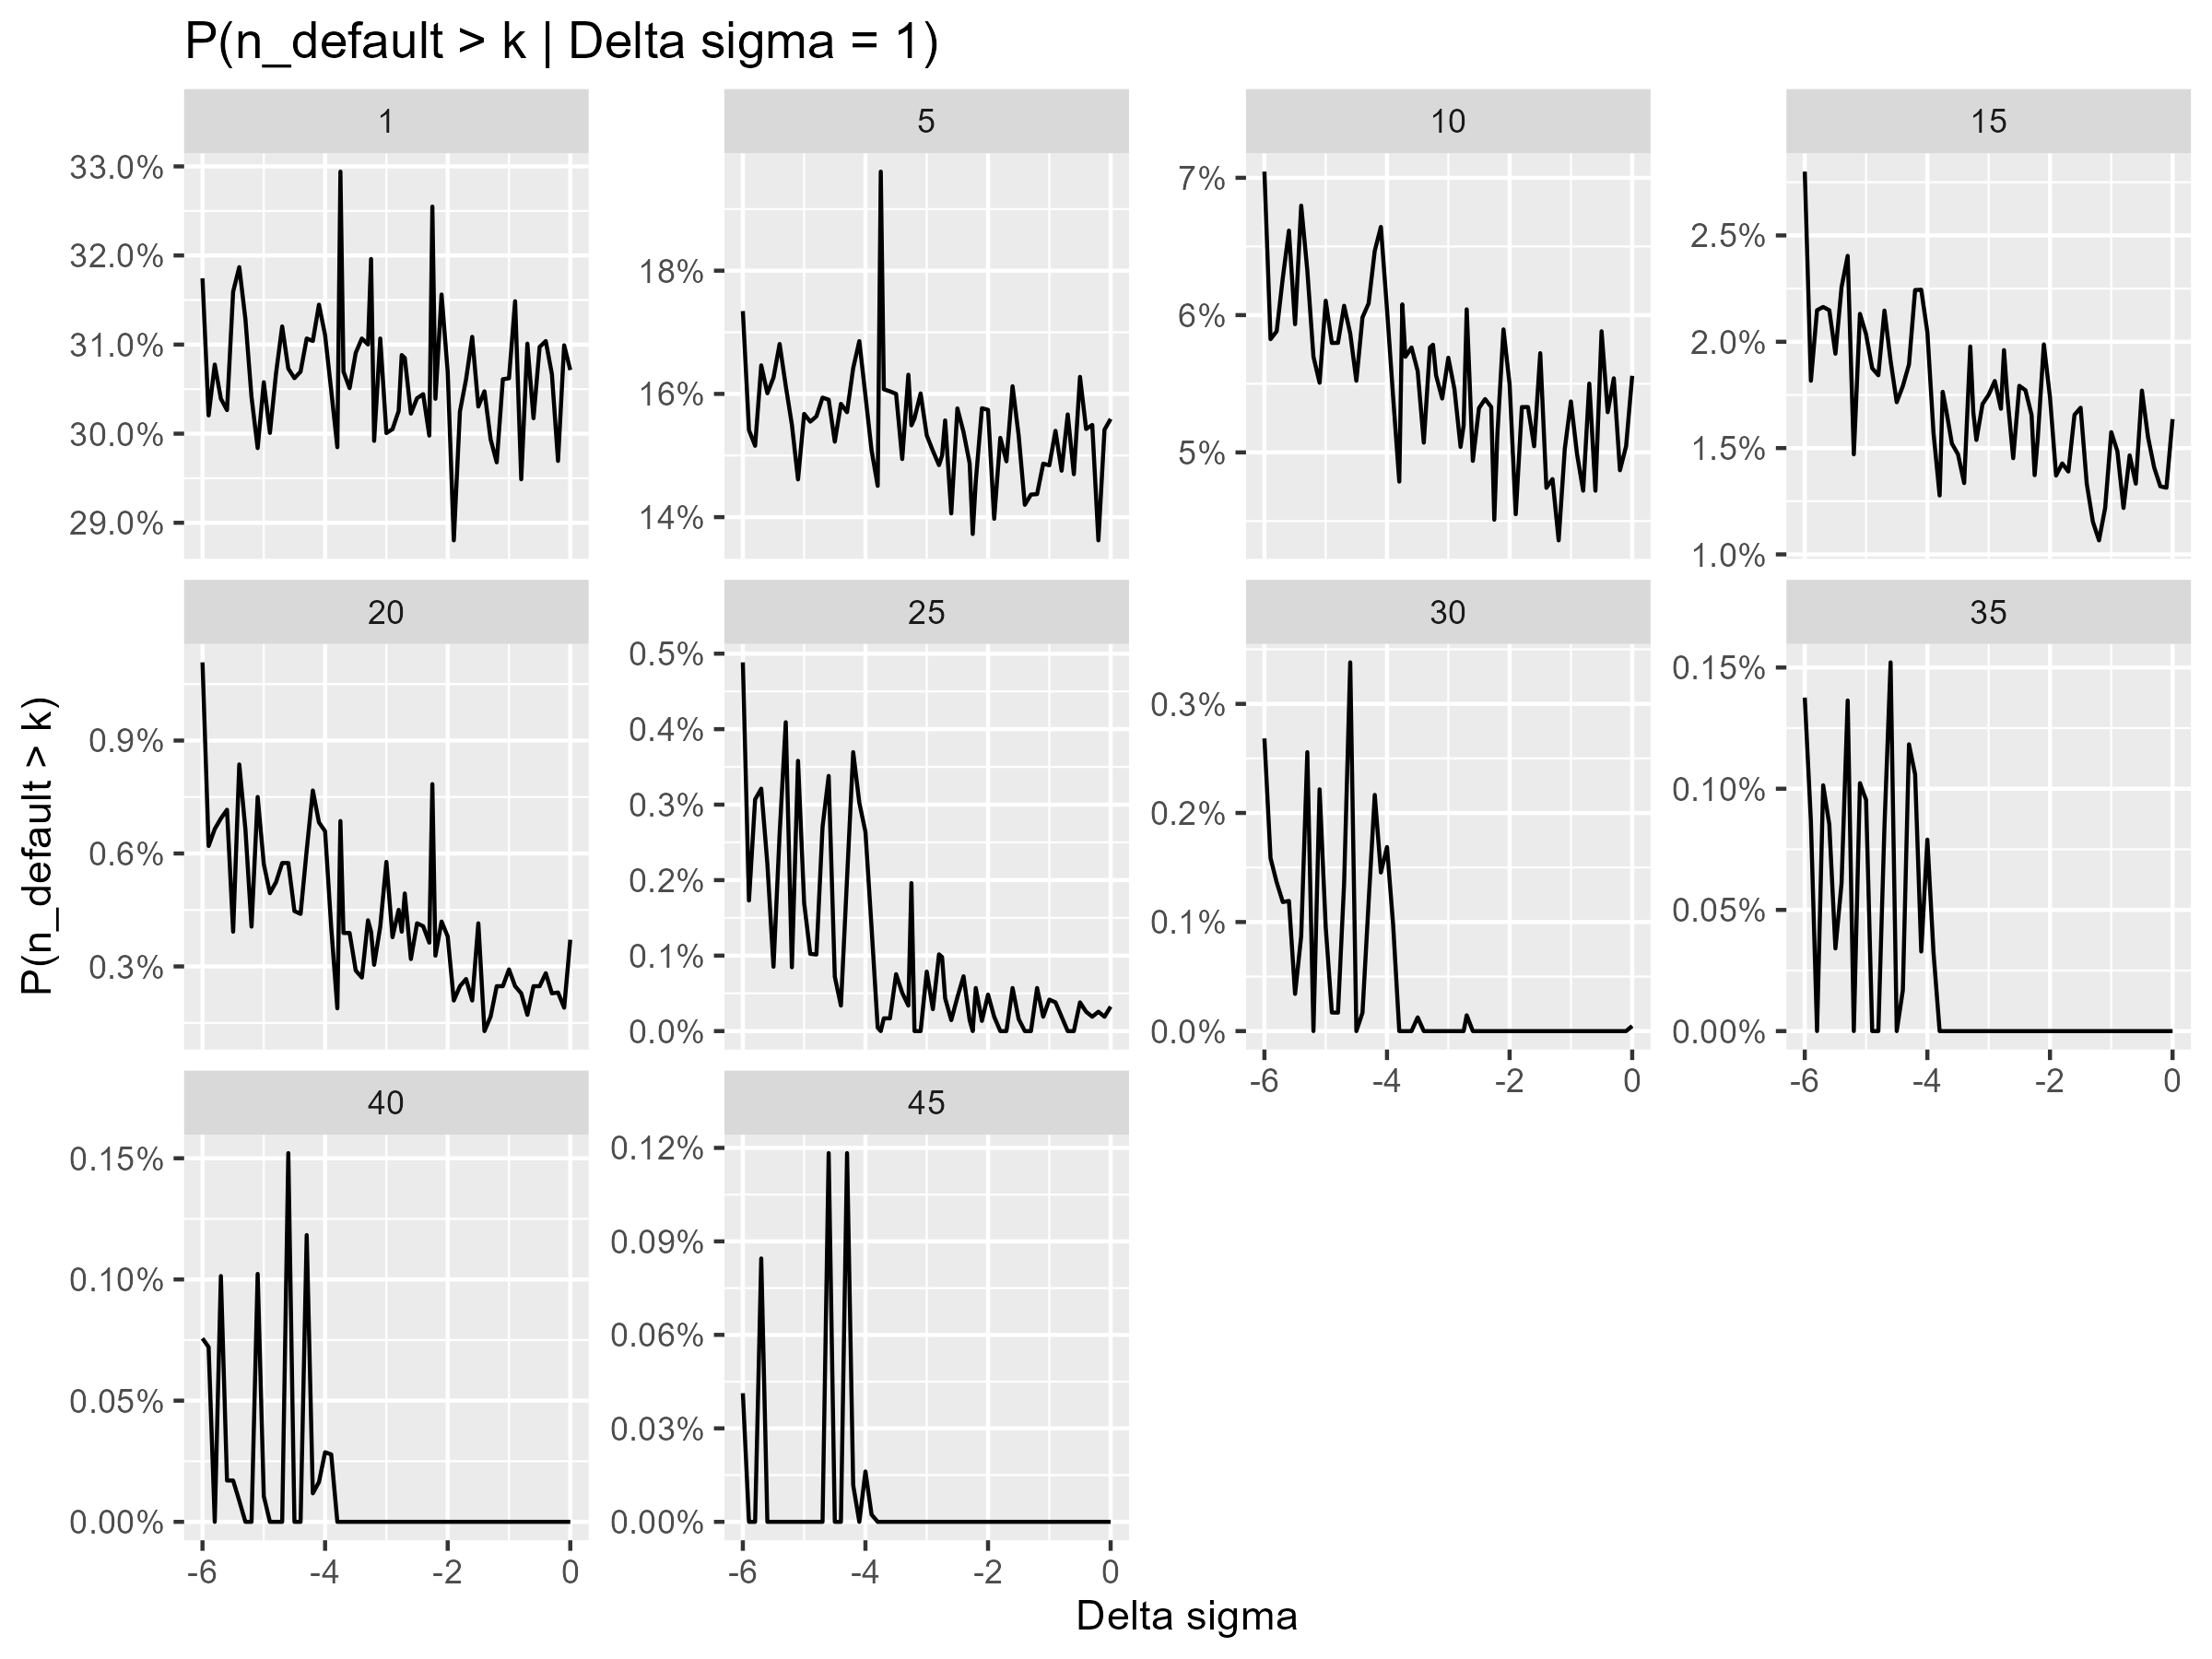
\includegraphics[scale=0.4]{more_than_plot.png}
        \centering
    \end{figure}  
      
    \end{frame}

% frame with references

\begin{frame}{References}

    
    \

    \begin{itemize}
        \item  Aldasoro, Iñaki and Delli Gatti, Domenico and Faia, Ester. "Bank networks: Contagion, systemic risk and prudential policy". Journal of Economic Behavior \& Organization, 2017, vol. 142, issue C, 164-188
        \item Bluhm, Marcel, and Jan-Pieter Krahnen. "Systemic risk in an interconnected banking system with endogenous asset markets." Journal of Financial Stability 13 (2014): 75-94.
        \item Regulation No 575/2013 of the European Parliament and of the Council of 26 June 2013 (Basel III implementation in Europe)
    \end{itemize}

\end{frame}

    
\end{document}

